% !TeX root = ../tesis.tex


\begin{figure}\centering
%\def\svgwidth{\textwidth} \small
%\includeinkscape{2-Results-Figs/redshift/redshift}%
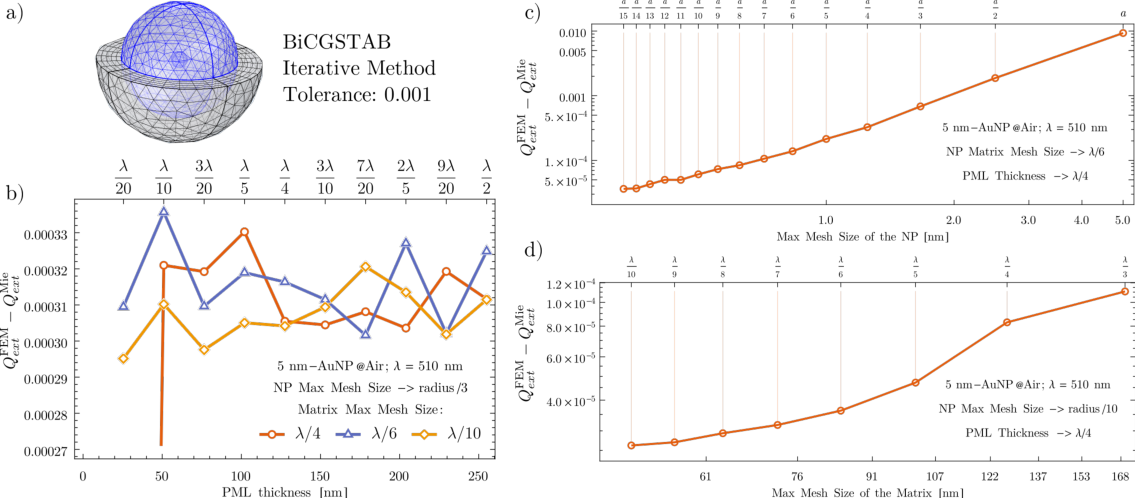
\includegraphics[scale = .8 ]{1-Theory-Figs/drawingCOMSOL.pdf}
\caption[Convergence tests: The Meshing]{Resonance wavlength ($\lambda_\text{res}$) of the scattering (orange) and extinction (black) cross sections as functions of the NPs radii when embedded  \ref{sfig:red:1} into air and \ref{sfig:red:2} into water, and as function of the refractive index of the matrix for NP of radius set to  \ref{sfig:red:3} 12.5 nm and \ref{sfig:red:4} 50 nm.}
\end{figure}

\clearpage

\begin{figure}\centering
%\def\svgwidth{\textwidth} \small
%\includeinkscape{2-Results-Figs/redshift/redshift}%
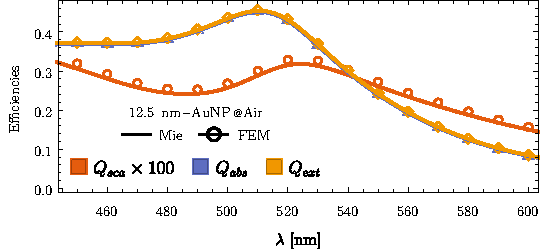
\includegraphics[width = .8\textwidth ]{1-Theory-Figs/Mie-FEM_Air.pdf}\\
\includegraphics[width = .4\textwidth ]{1-Theory-Figs/Isolated-COMSOL.pdf}%
\includegraphics[width = .4\textwidth ]{1-Theory-Figs/Isolated-COMSOL.pdf}%
\caption[Convergence tests: The Meshing]{Resonance wavlength ($\lambda_\text{res}$) of the scattering (orange) and extinction (black) cross sections as functions of the NPs radii when embedded  \ref{sfig:red:1} into air and \ref{sfig:red:2} into water, and as function of the refractive index of the matrix for NP of radius set to  \ref{sfig:red:3} 12.5 nm and \ref{sfig:red:4} 50 nm.}
\end{figure}
































